\section{Application}
During the first sprint, we started development on the application.
The following features were implemented:
\begin{itemize}
    \item Login screen
    \item Application selection screen
    \item Create application screen
    \item Create user screen
    \item Task dashboard screen
    \item Create task screen
\end{itemize}

In this sprint, some of the functionality was mocked, because they were yet to be developed on the backend.
This was however limited to task functionality, where the rest was actual data transmitted from the API.

\subsection{Design}
\label{sprint_1_design}
In the start of this sprint, some views were designed to give an idea of how the application should look.
The designs relevant to the features developed in this sprint.

The screens were designed to have a generic look, and feel familiar.
The tasks screen, which can be seen on ~\autoref{task_dashboard_screen}, was designed to look like a kanban board \cite{kanbanBoard}.
This was done because Kanban boards are a common way to organize tasks.

\begin{figure}[H]
    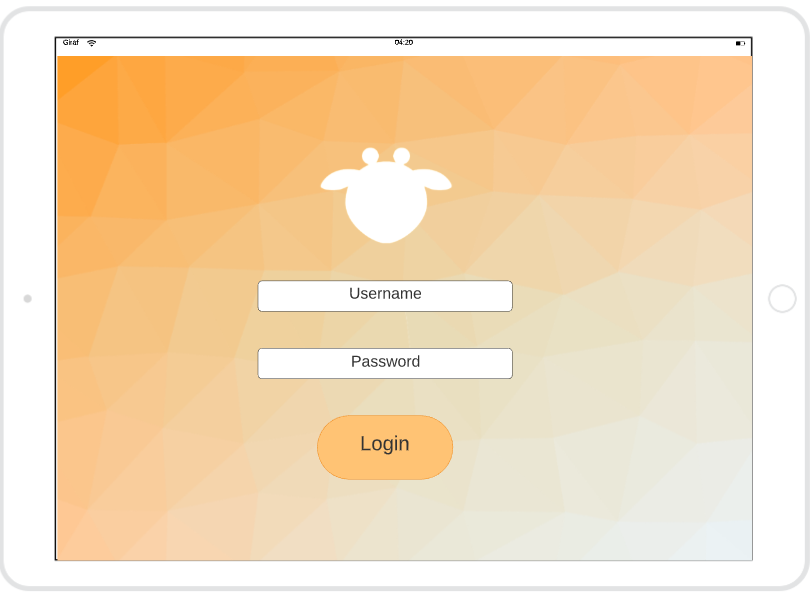
\includegraphics[width=\textwidth]{Sprint_1/images/login_screen.png}
    \caption{Login screen design.}
    \label{login_screen_design}
\end{figure}

\begin{figure}[H]
    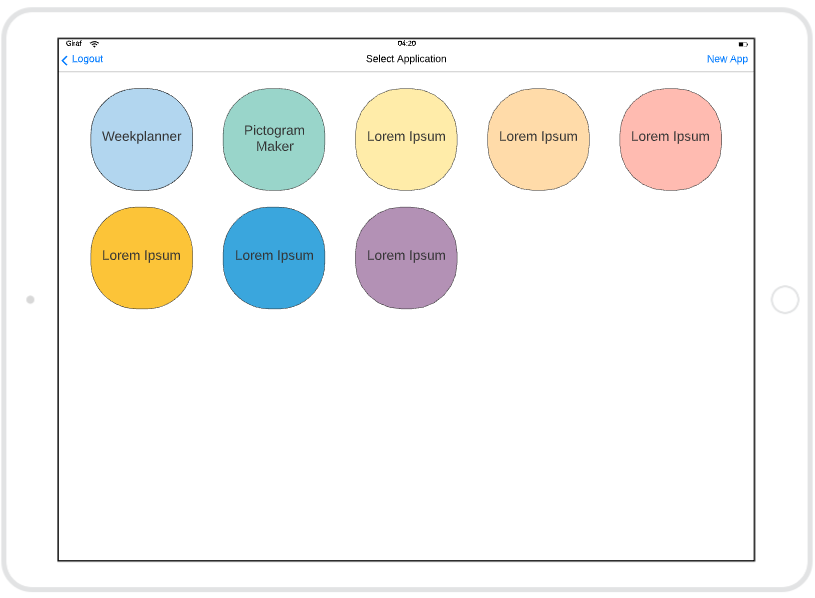
\includegraphics[width=\textwidth]{Sprint_1/images/app_selection_screen.png}
    \caption{Application selection screen design.}
    \label{app_selection_screen}

\end{figure}

\begin{figure}[H]
    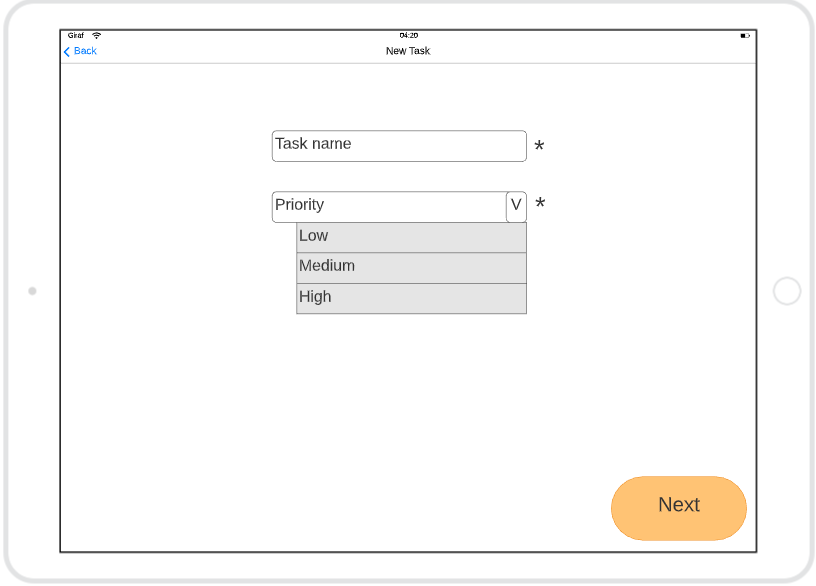
\includegraphics[width=\textwidth]{Sprint_1/images/create_task_screen.png}
    \caption{Create task screen design.}
    \label{create_task_screen}

\end{figure}

\begin{figure}[H]
    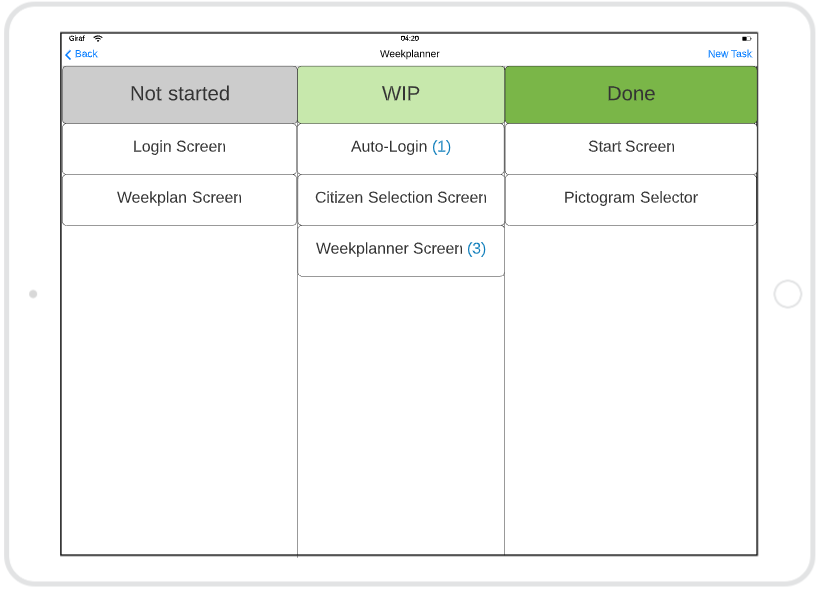
\includegraphics[width=\textwidth]{Sprint_1/images/task_dashboard_screen.png}
    \caption{Task dashboard screen design.}
    \label{task_dashboard_screen}
\end{figure}

\subsection{Implementation}
Most of this sprint was used on setting up the project and some code was written to allow for easier future development.
This includes a base screen that all other screens should extend, which adds nice-to-have functionality such as detecting if the device is a tablet or phone, and if it is in portrait or landscape mode.

The screens shown in~\autoref{sprint_1_design} have been implemented, and screenshots of the implementations can be seen in~\autoref{login_screen_design_app},~\autoref{app_selection_screen_app},~\autoref{app_creation_screen_app}, ~\autoref{create_task_screen_app} and~\autoref{task_dashboard_screen_app}.

The screens implemented have the needed functionality, but no tasks are shown in the Task screen~(~\autoref{task_dashboard_screen_app}), because this functionality was not yet implemented in the API.
But the application is ready for when this is implemented in Sprint 2.

The application code currently features all functionality available in the API as of Sprint 1.
However it is not all code that is used, but this makes it easy to implement new functionality without the need for implementing more API specific code. 

\begin{figure}[H]
    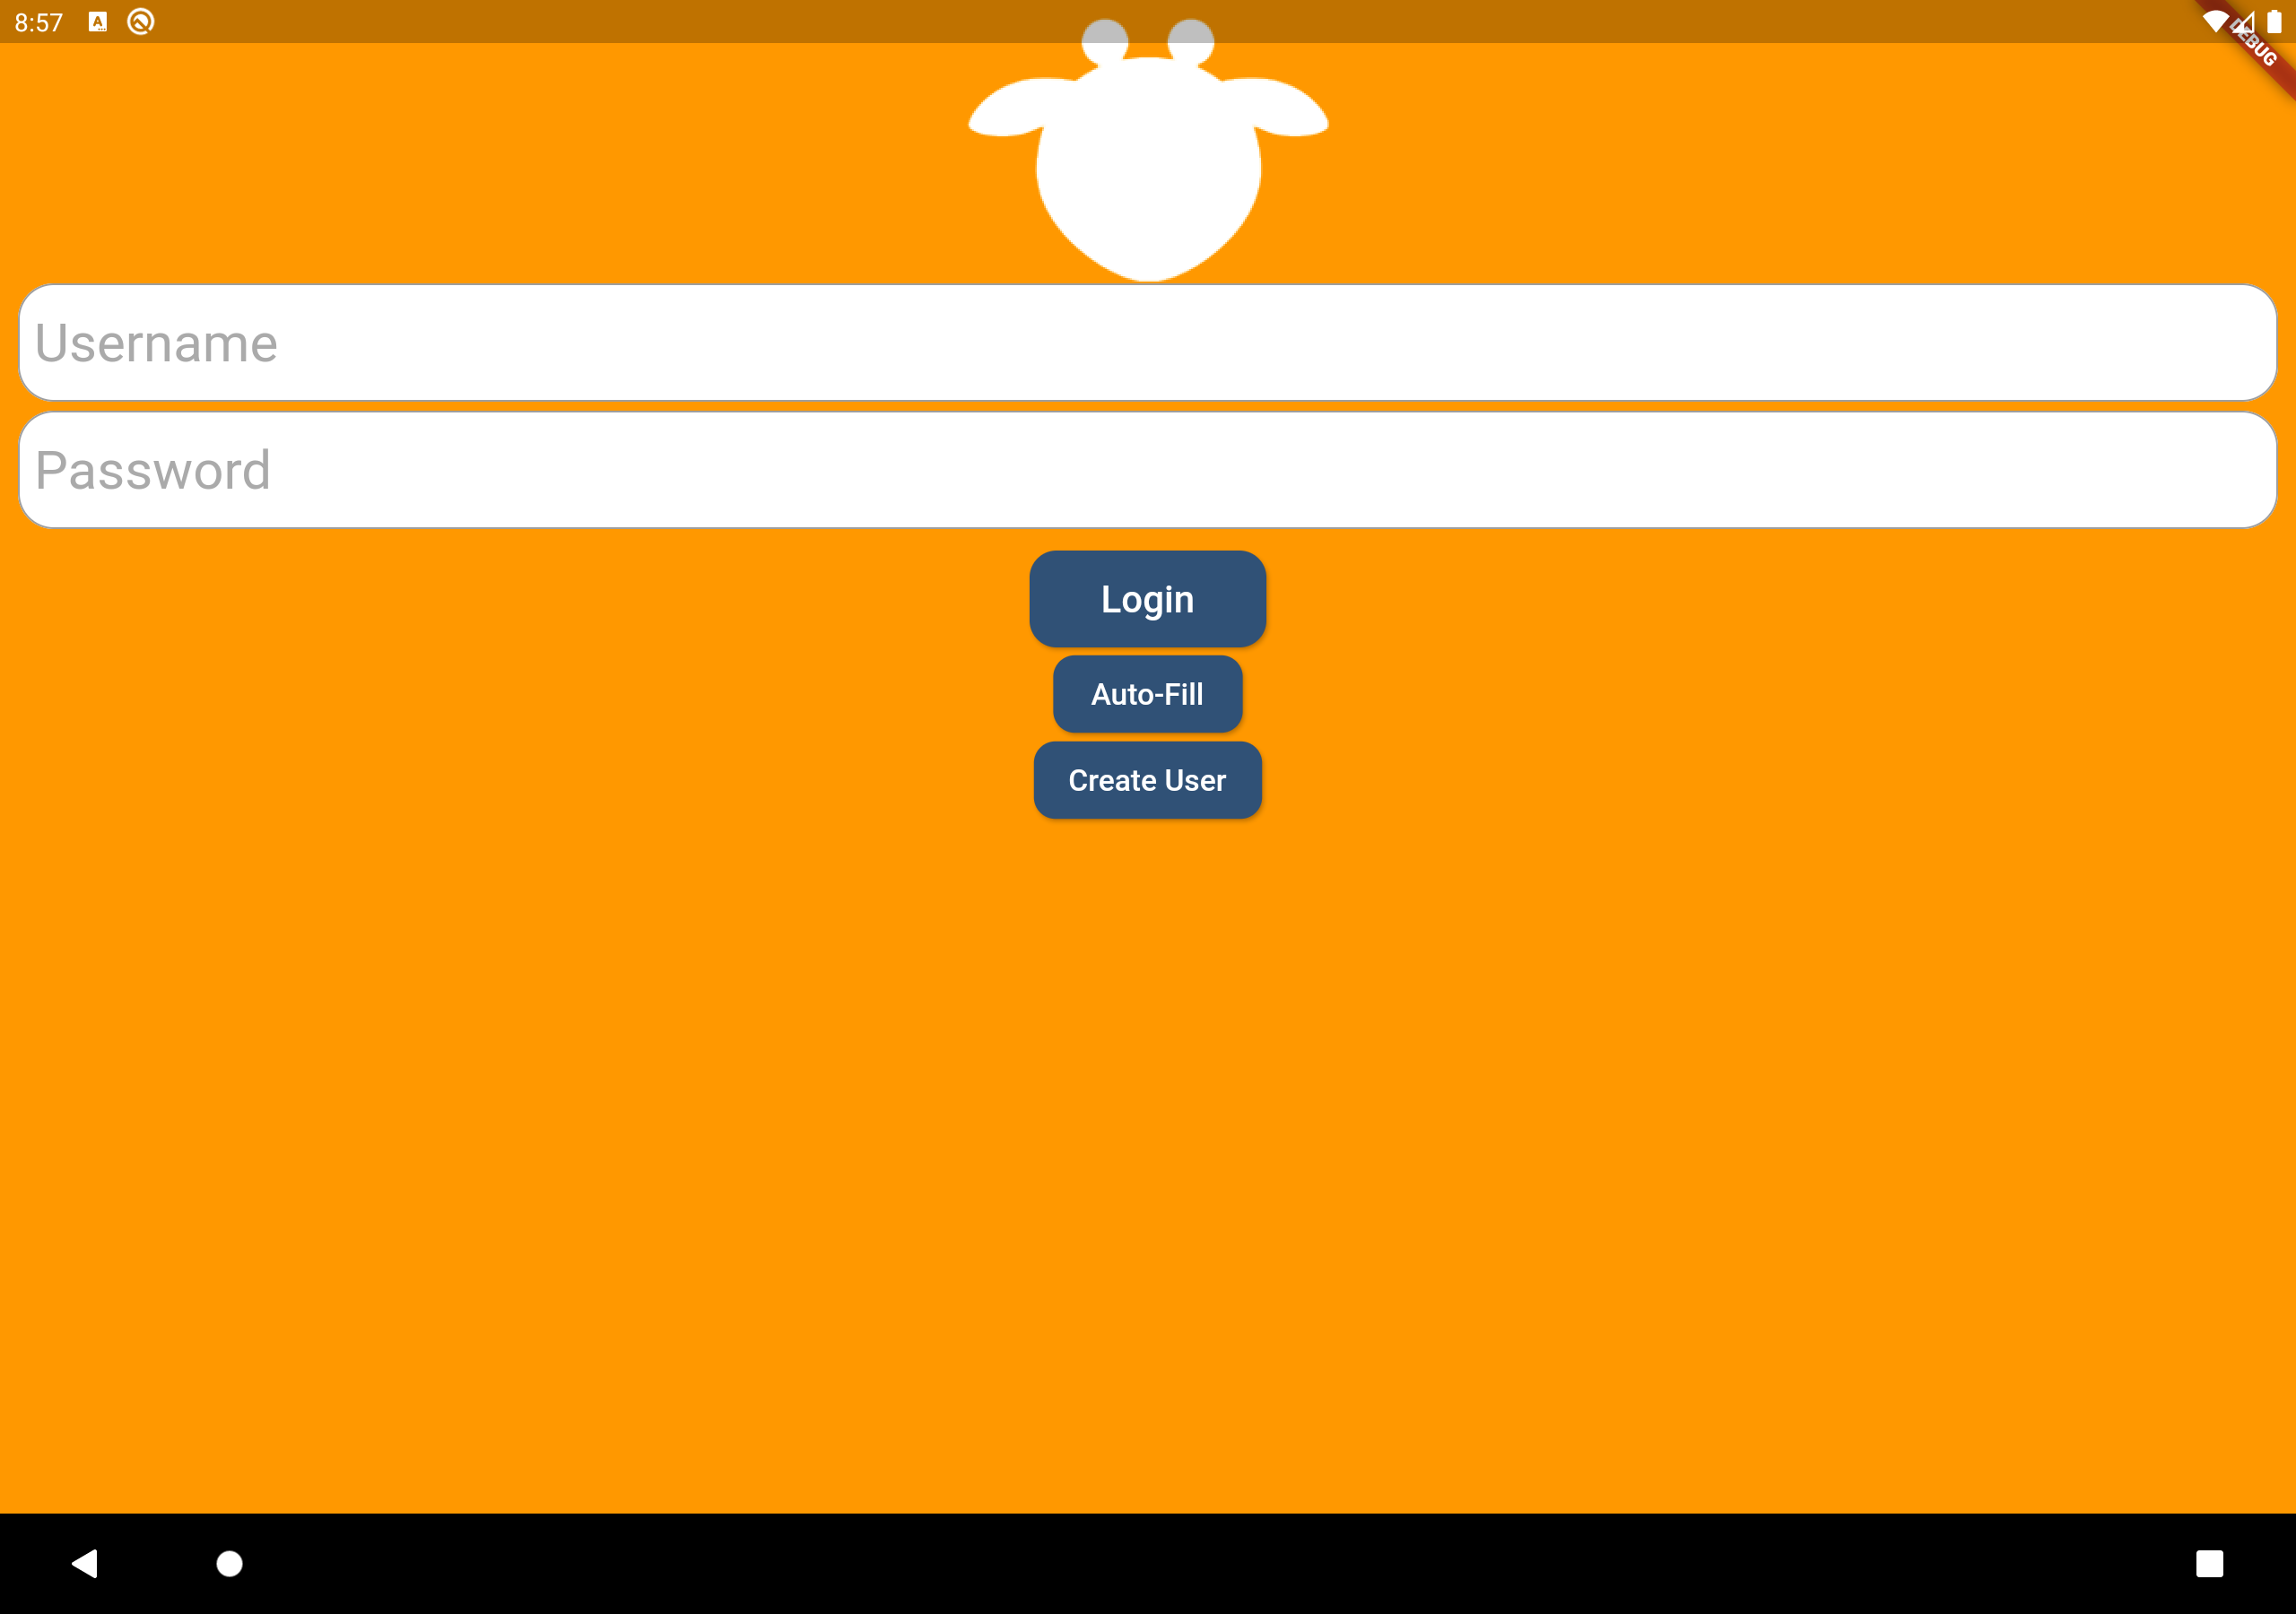
\includegraphics[width=\textwidth]{Sprint_1/images/login_screen_app.png}
    \caption{Login screen implementation.}
    \label{login_screen_design_app}
\end{figure}

\begin{figure}[H]
    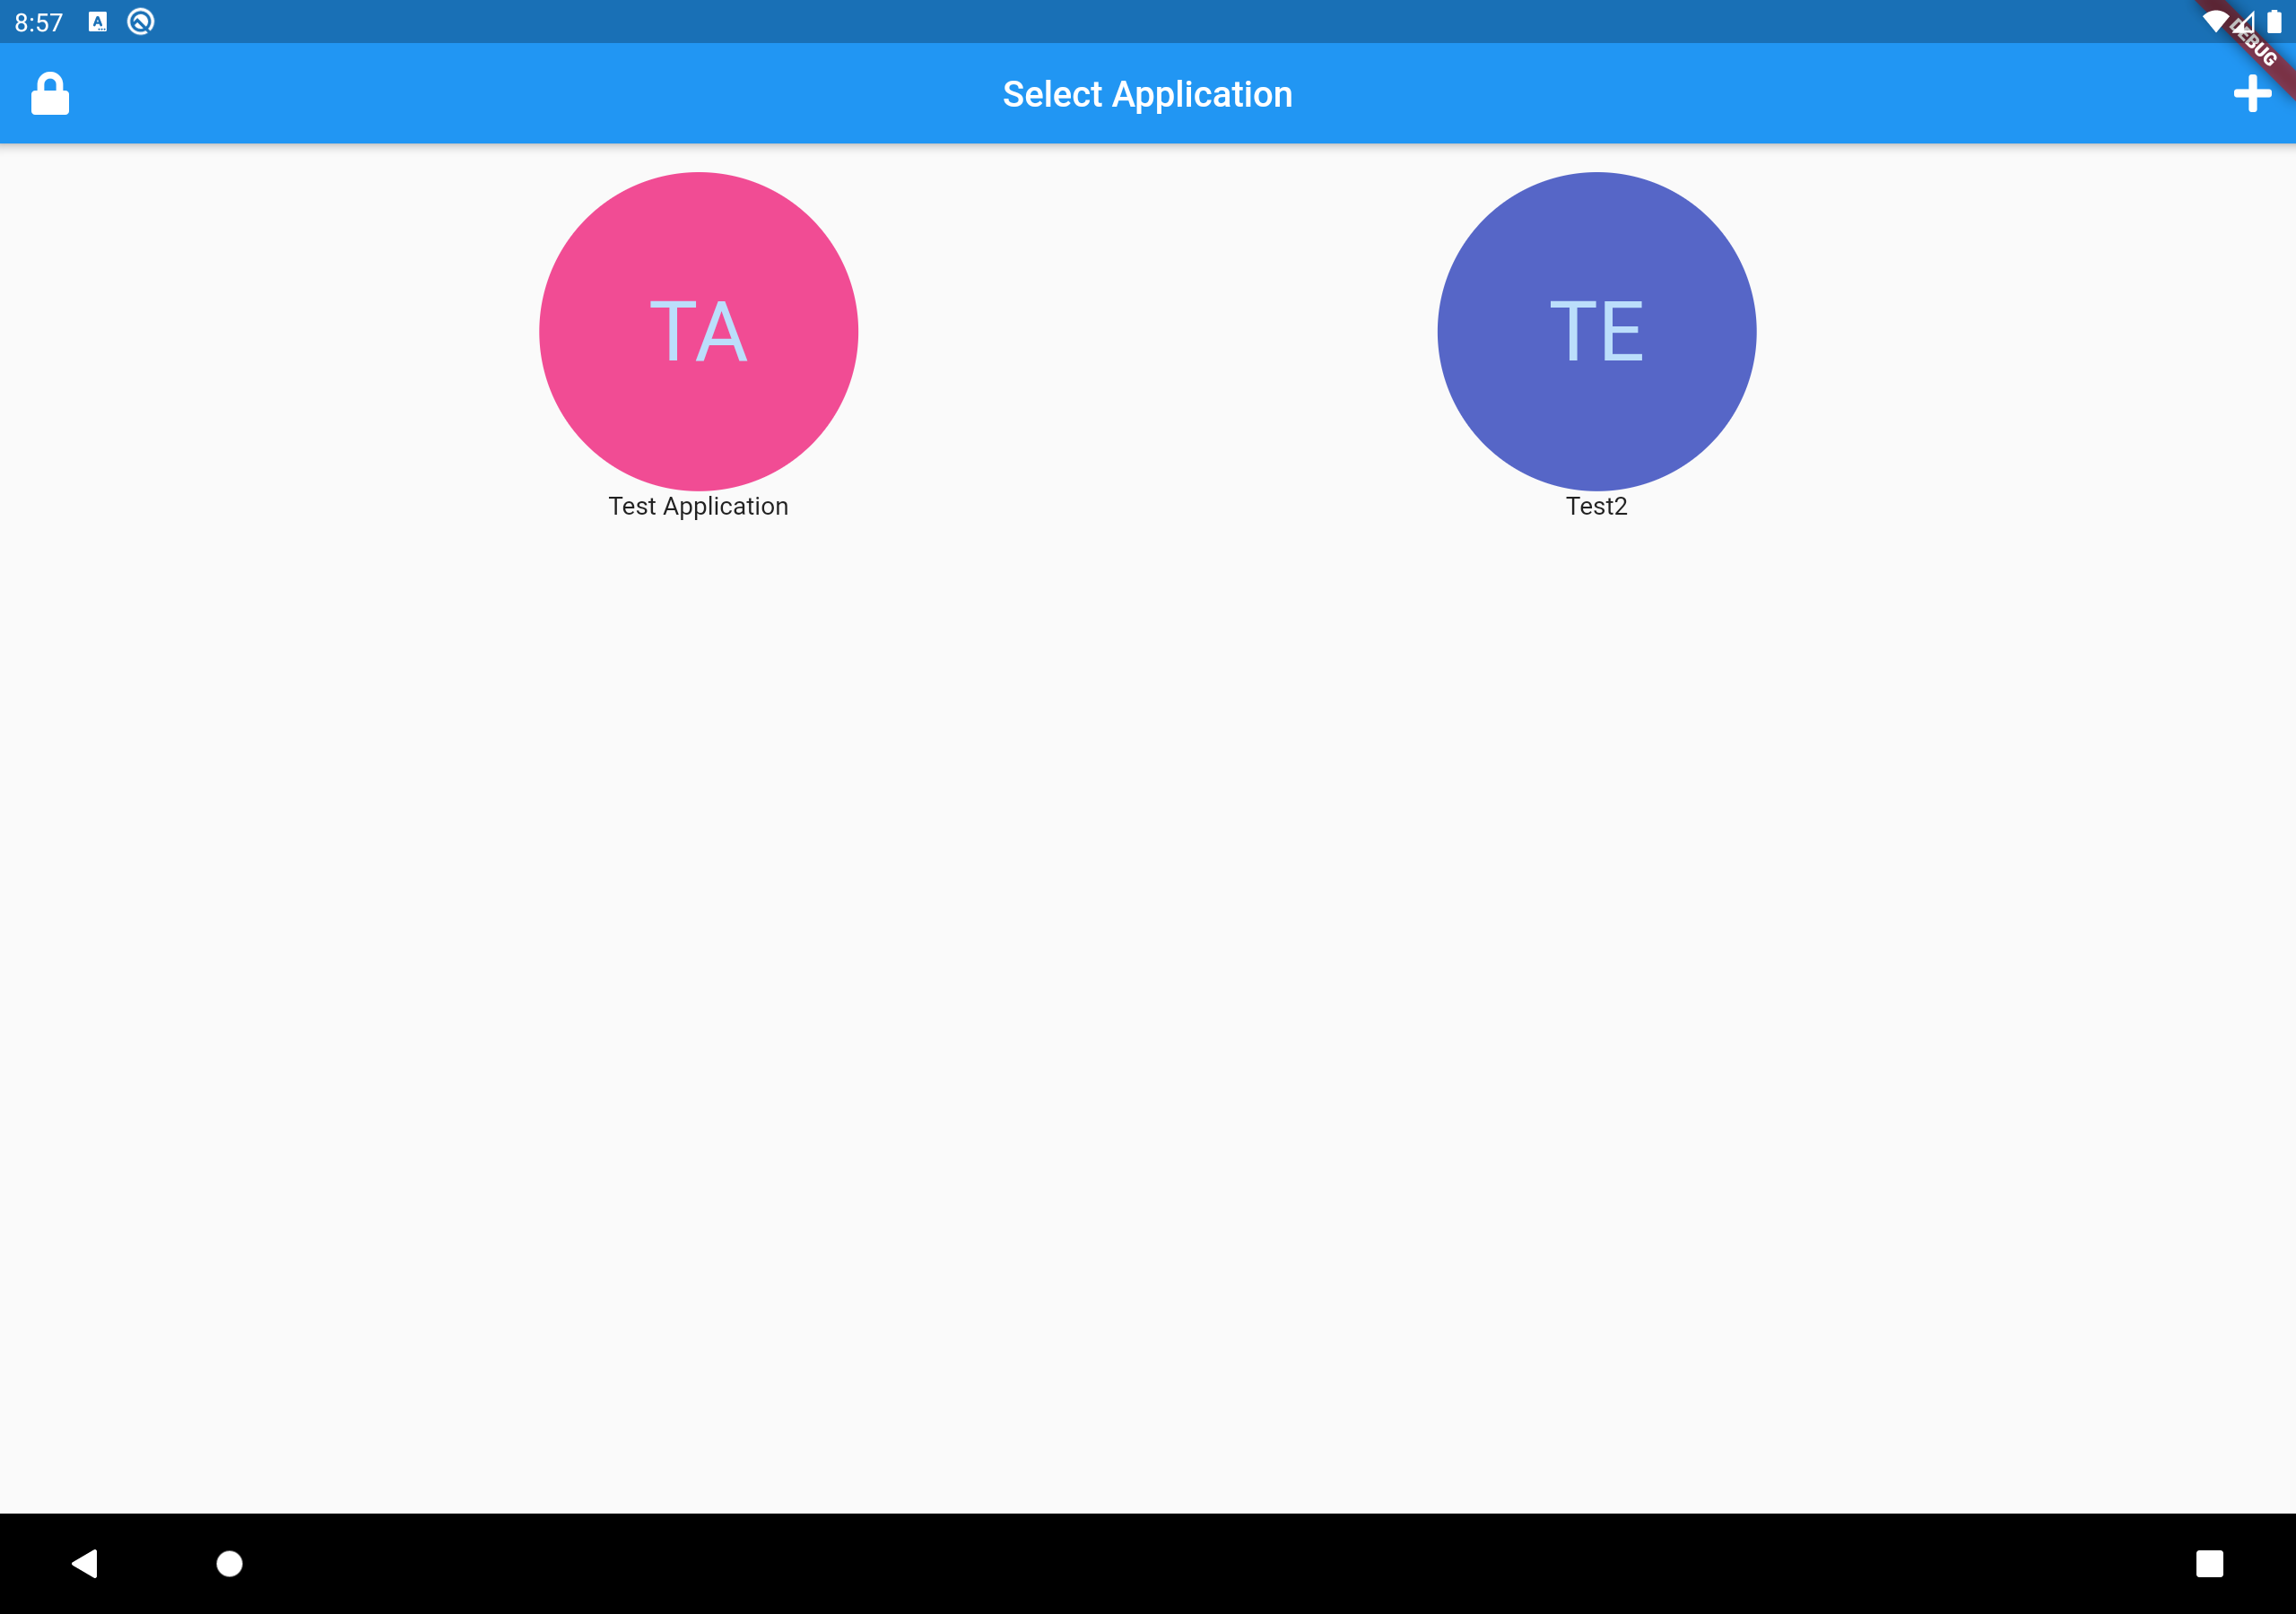
\includegraphics[width=\textwidth]{Sprint_1/images/app_selection_screen_app.png}
    \caption{Application selection screen implementation.}
    \label{app_selection_screen_app}
\end{figure}

\begin{figure}[H]
    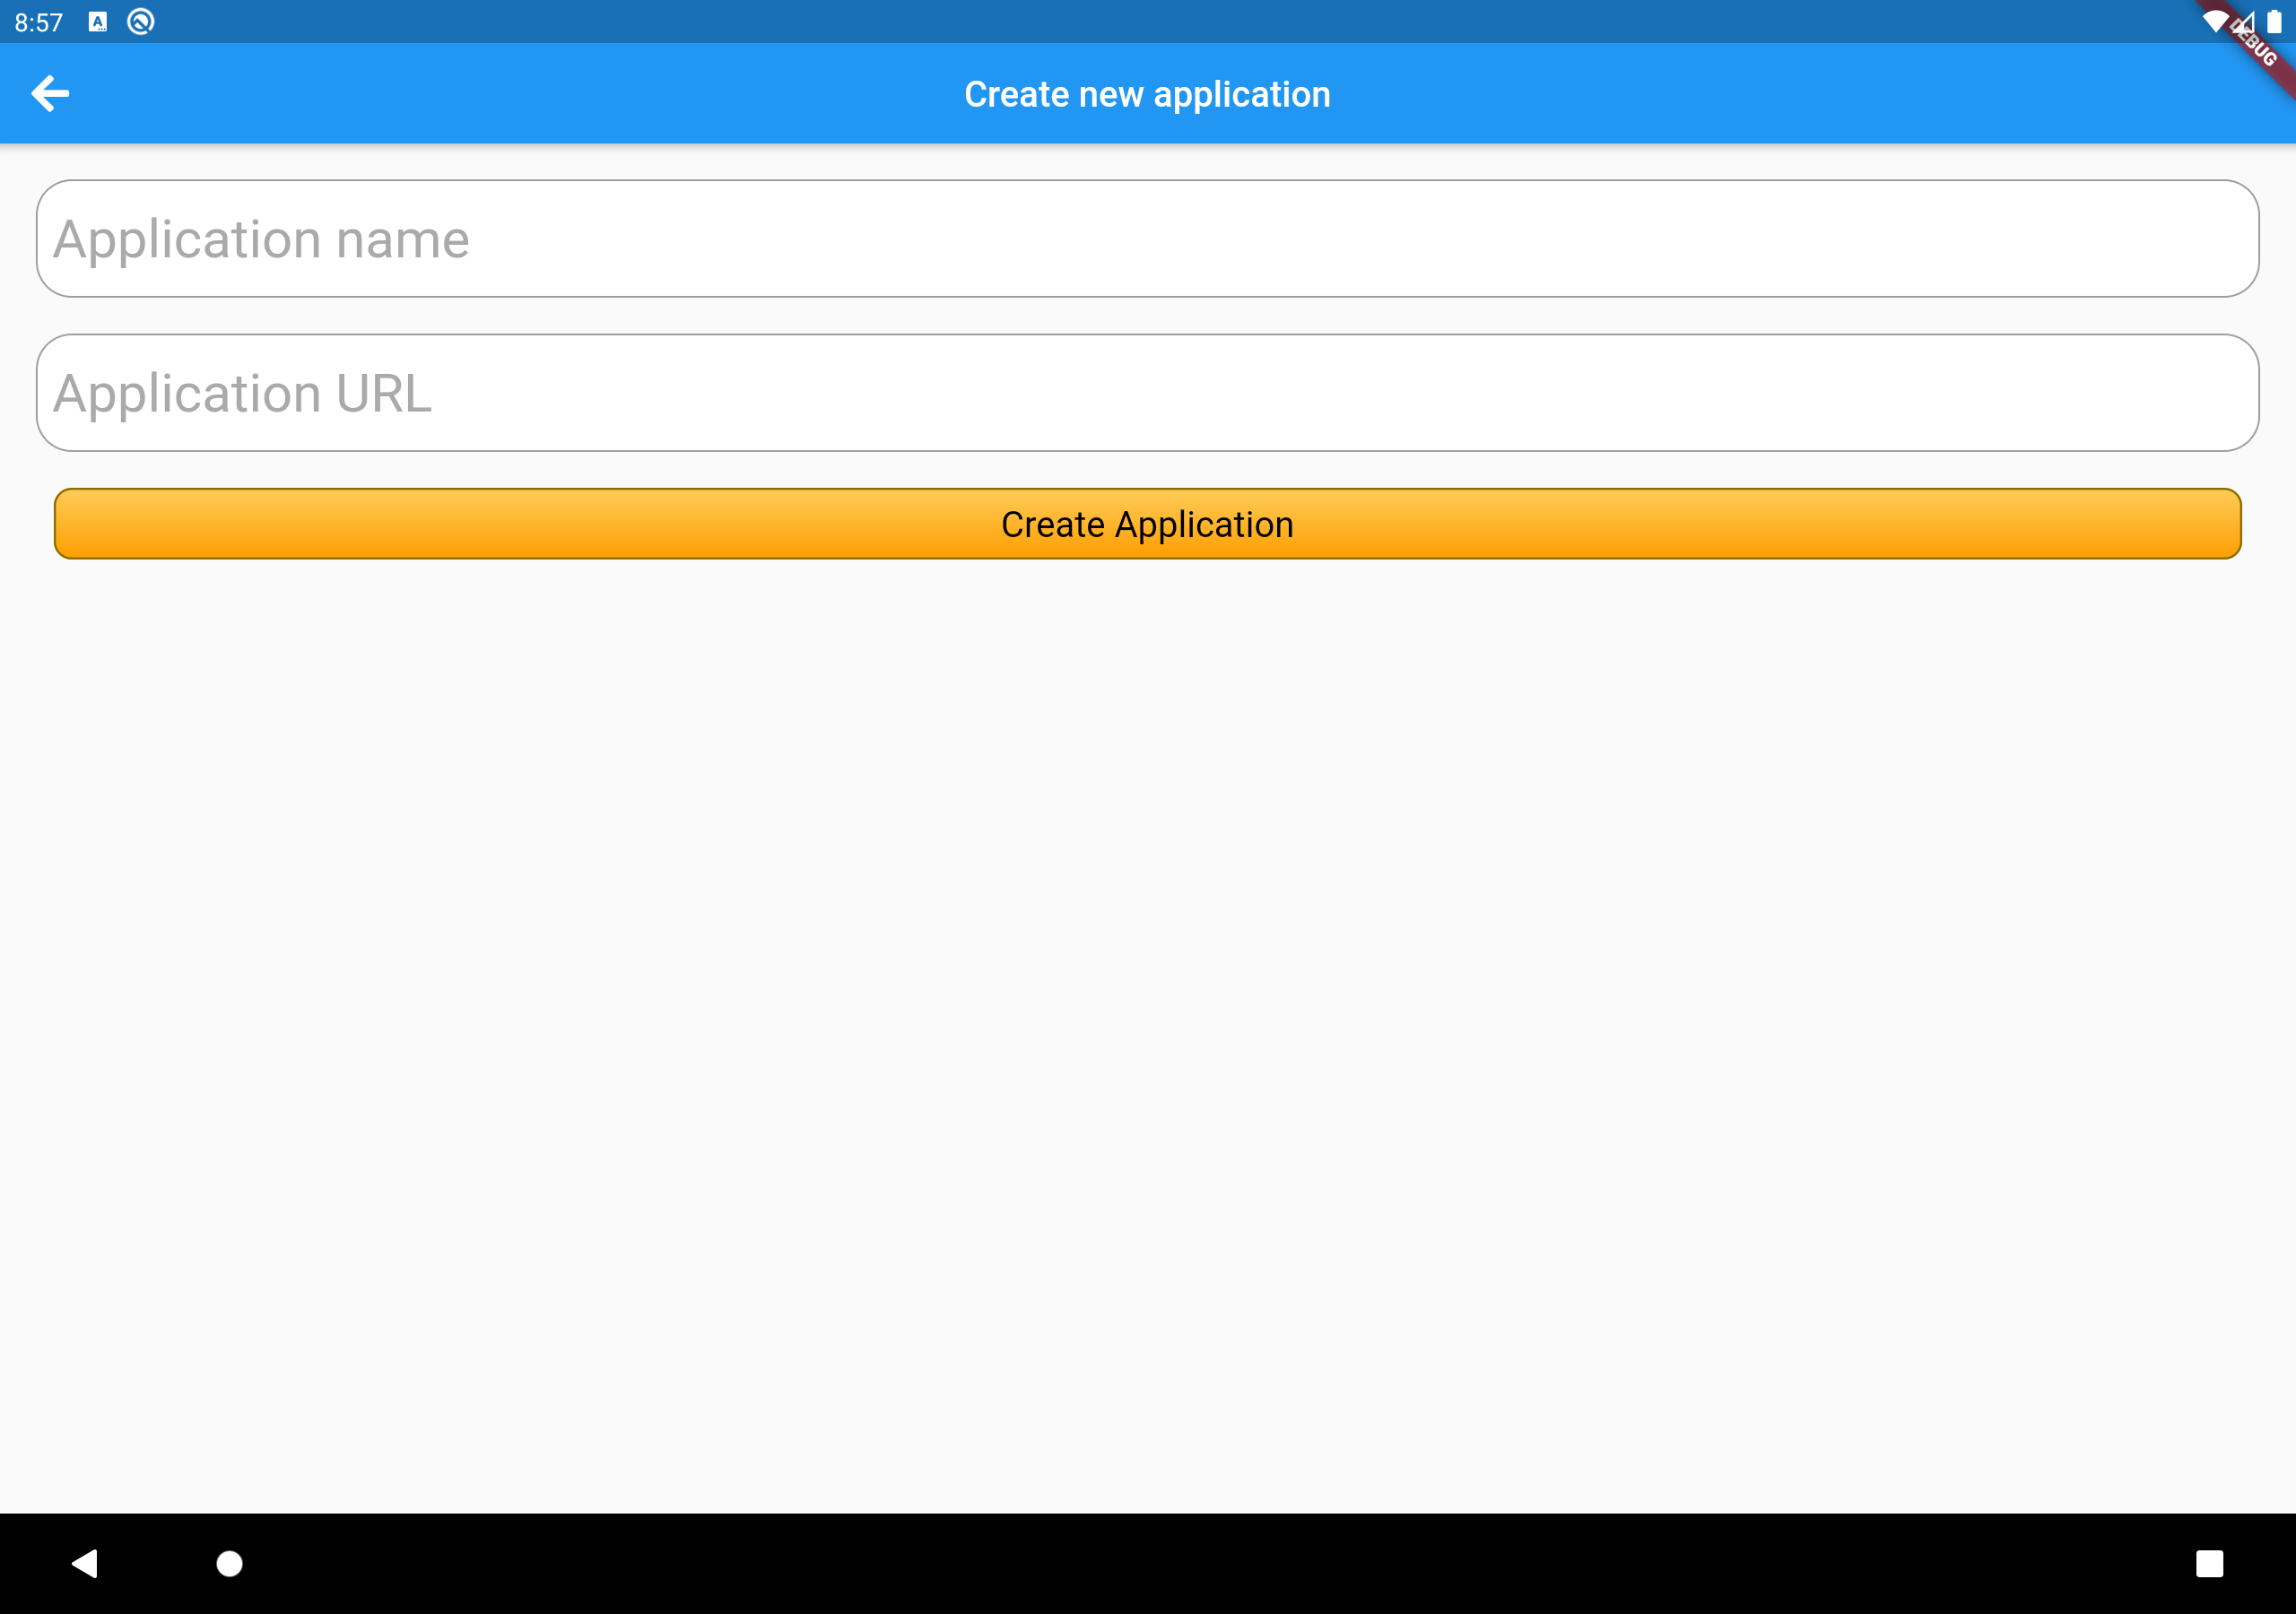
\includegraphics[width=\textwidth]{Sprint_1/images/create_app_screen_app.png}
    \caption{Application creation screen implementation.}
    \label{app_creation_screen_app}
\end{figure}

\begin{figure}[H]
    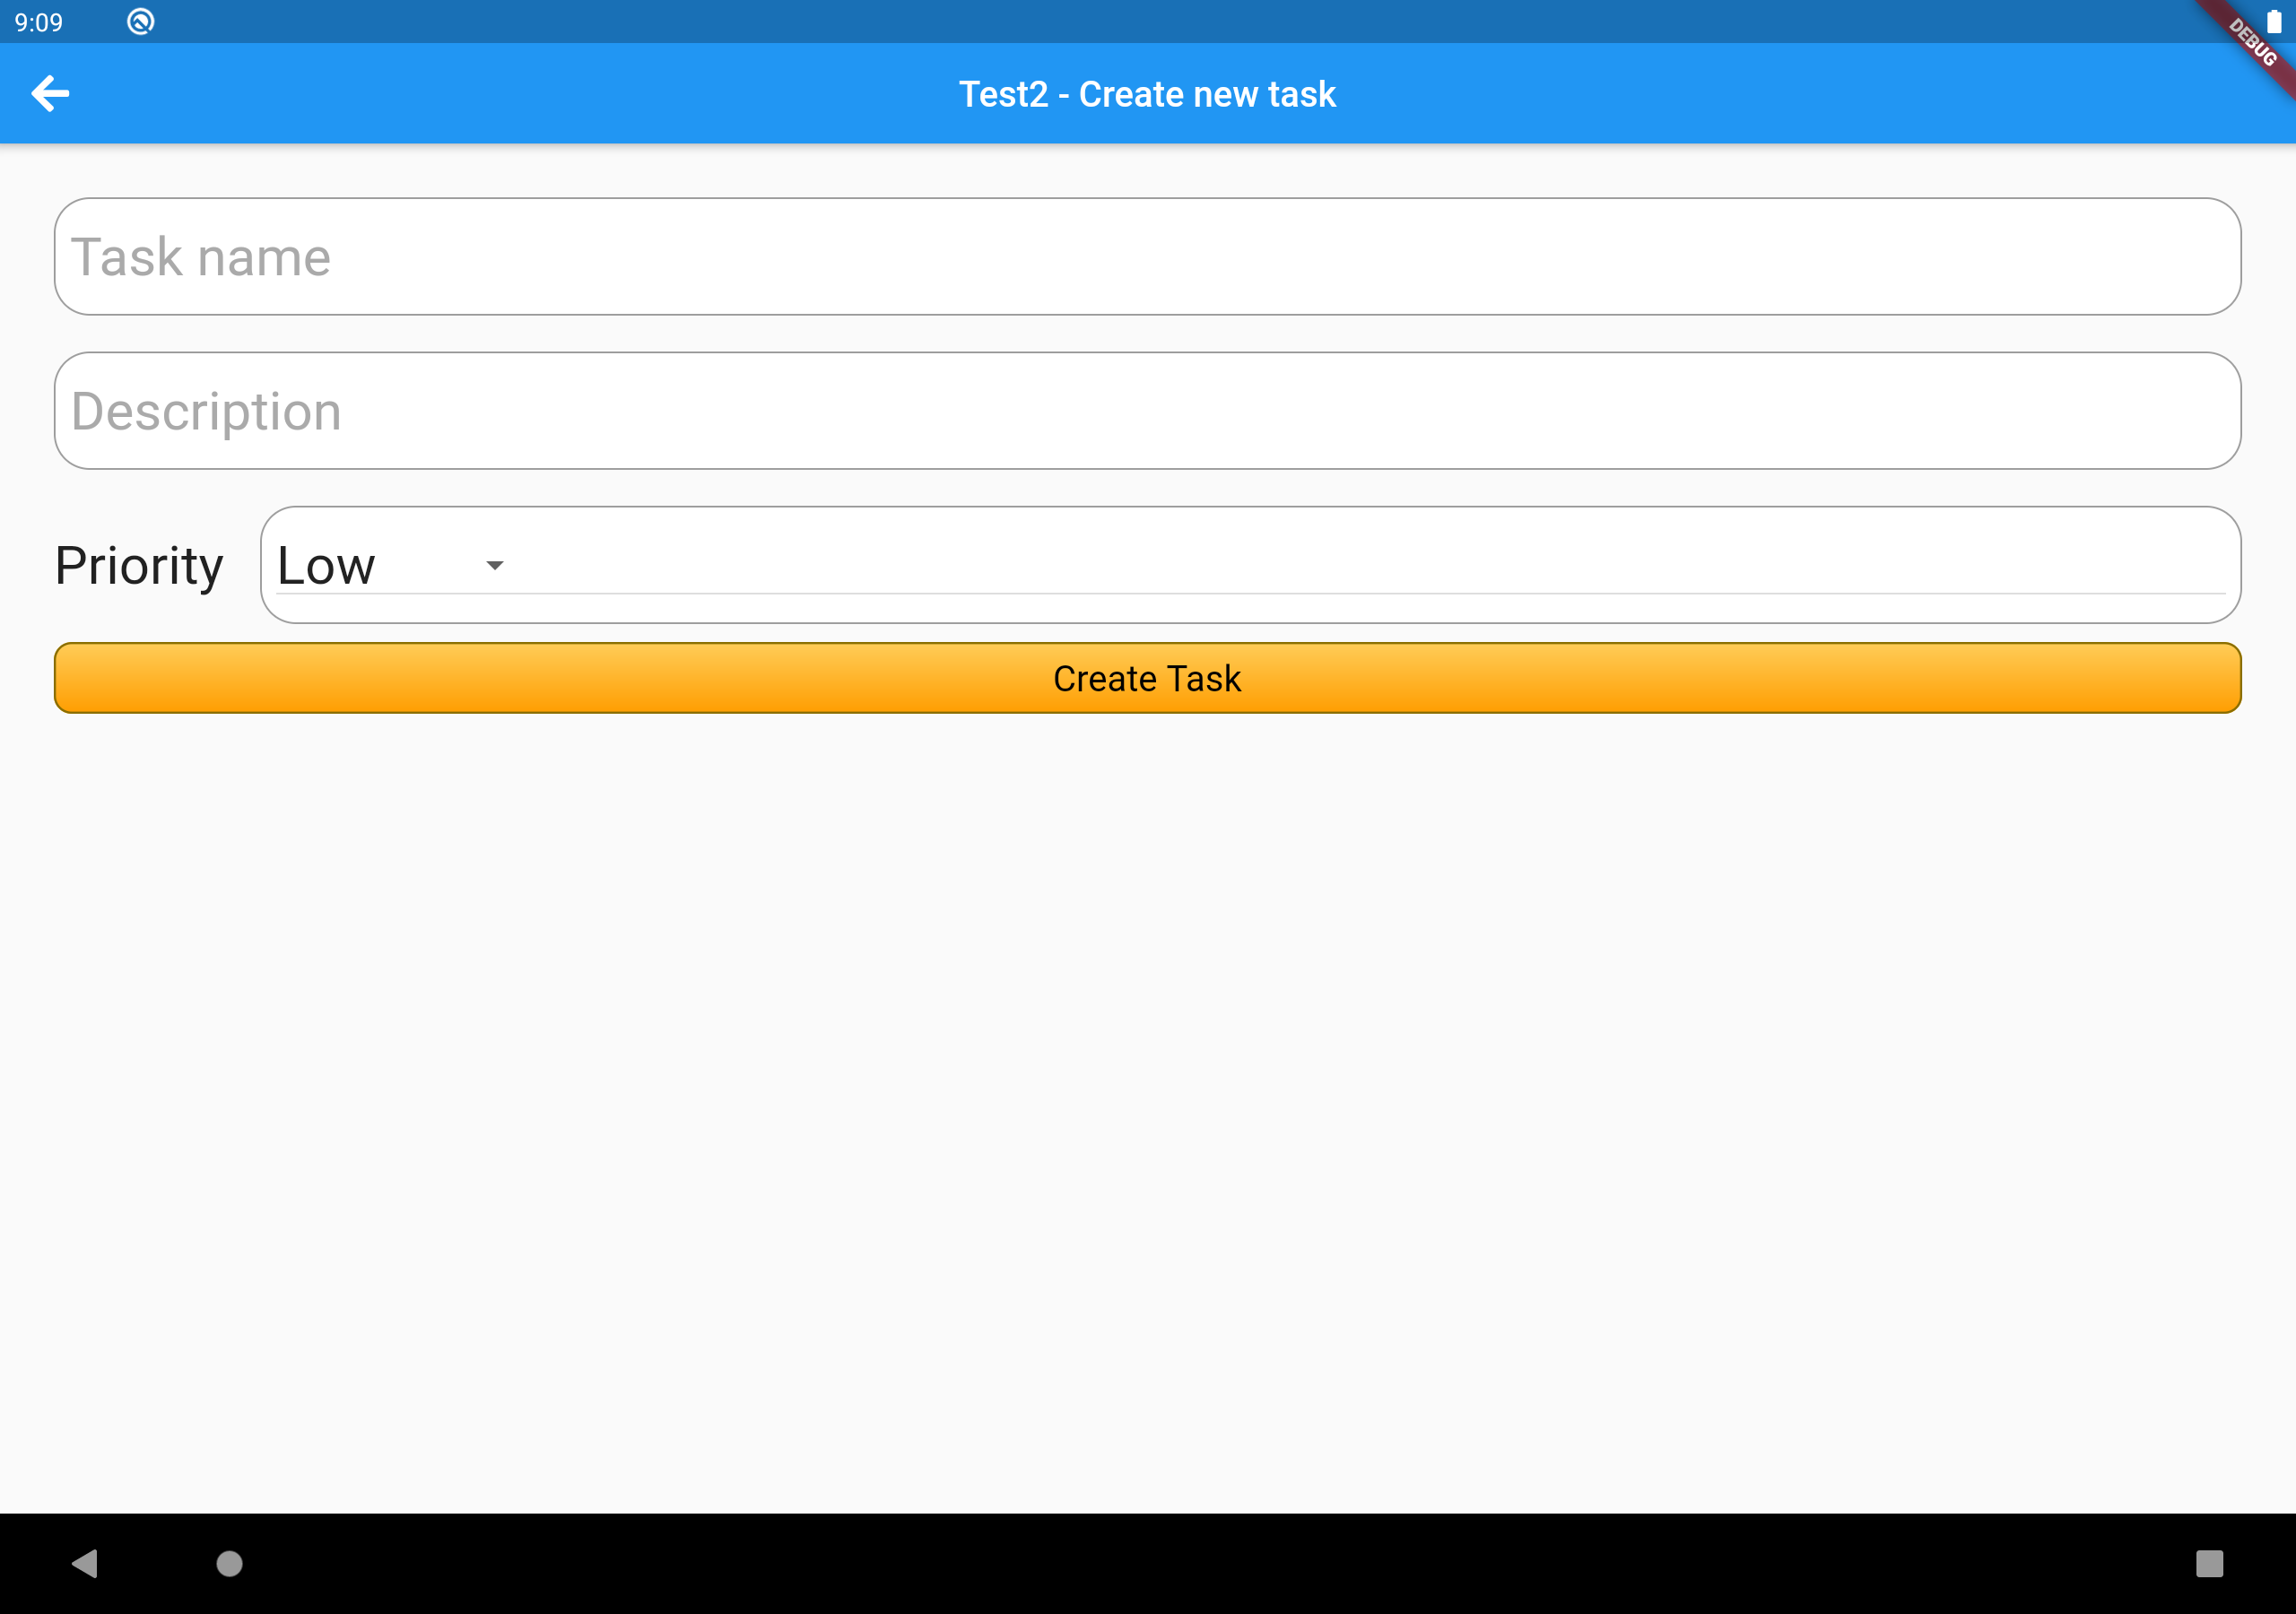
\includegraphics[width=\textwidth]{Sprint_1/images/create_task_screen_app.png}
    \caption{Create task screen implementation.}
    \label{create_task_screen_app}

\end{figure}

\begin{figure}[H]
    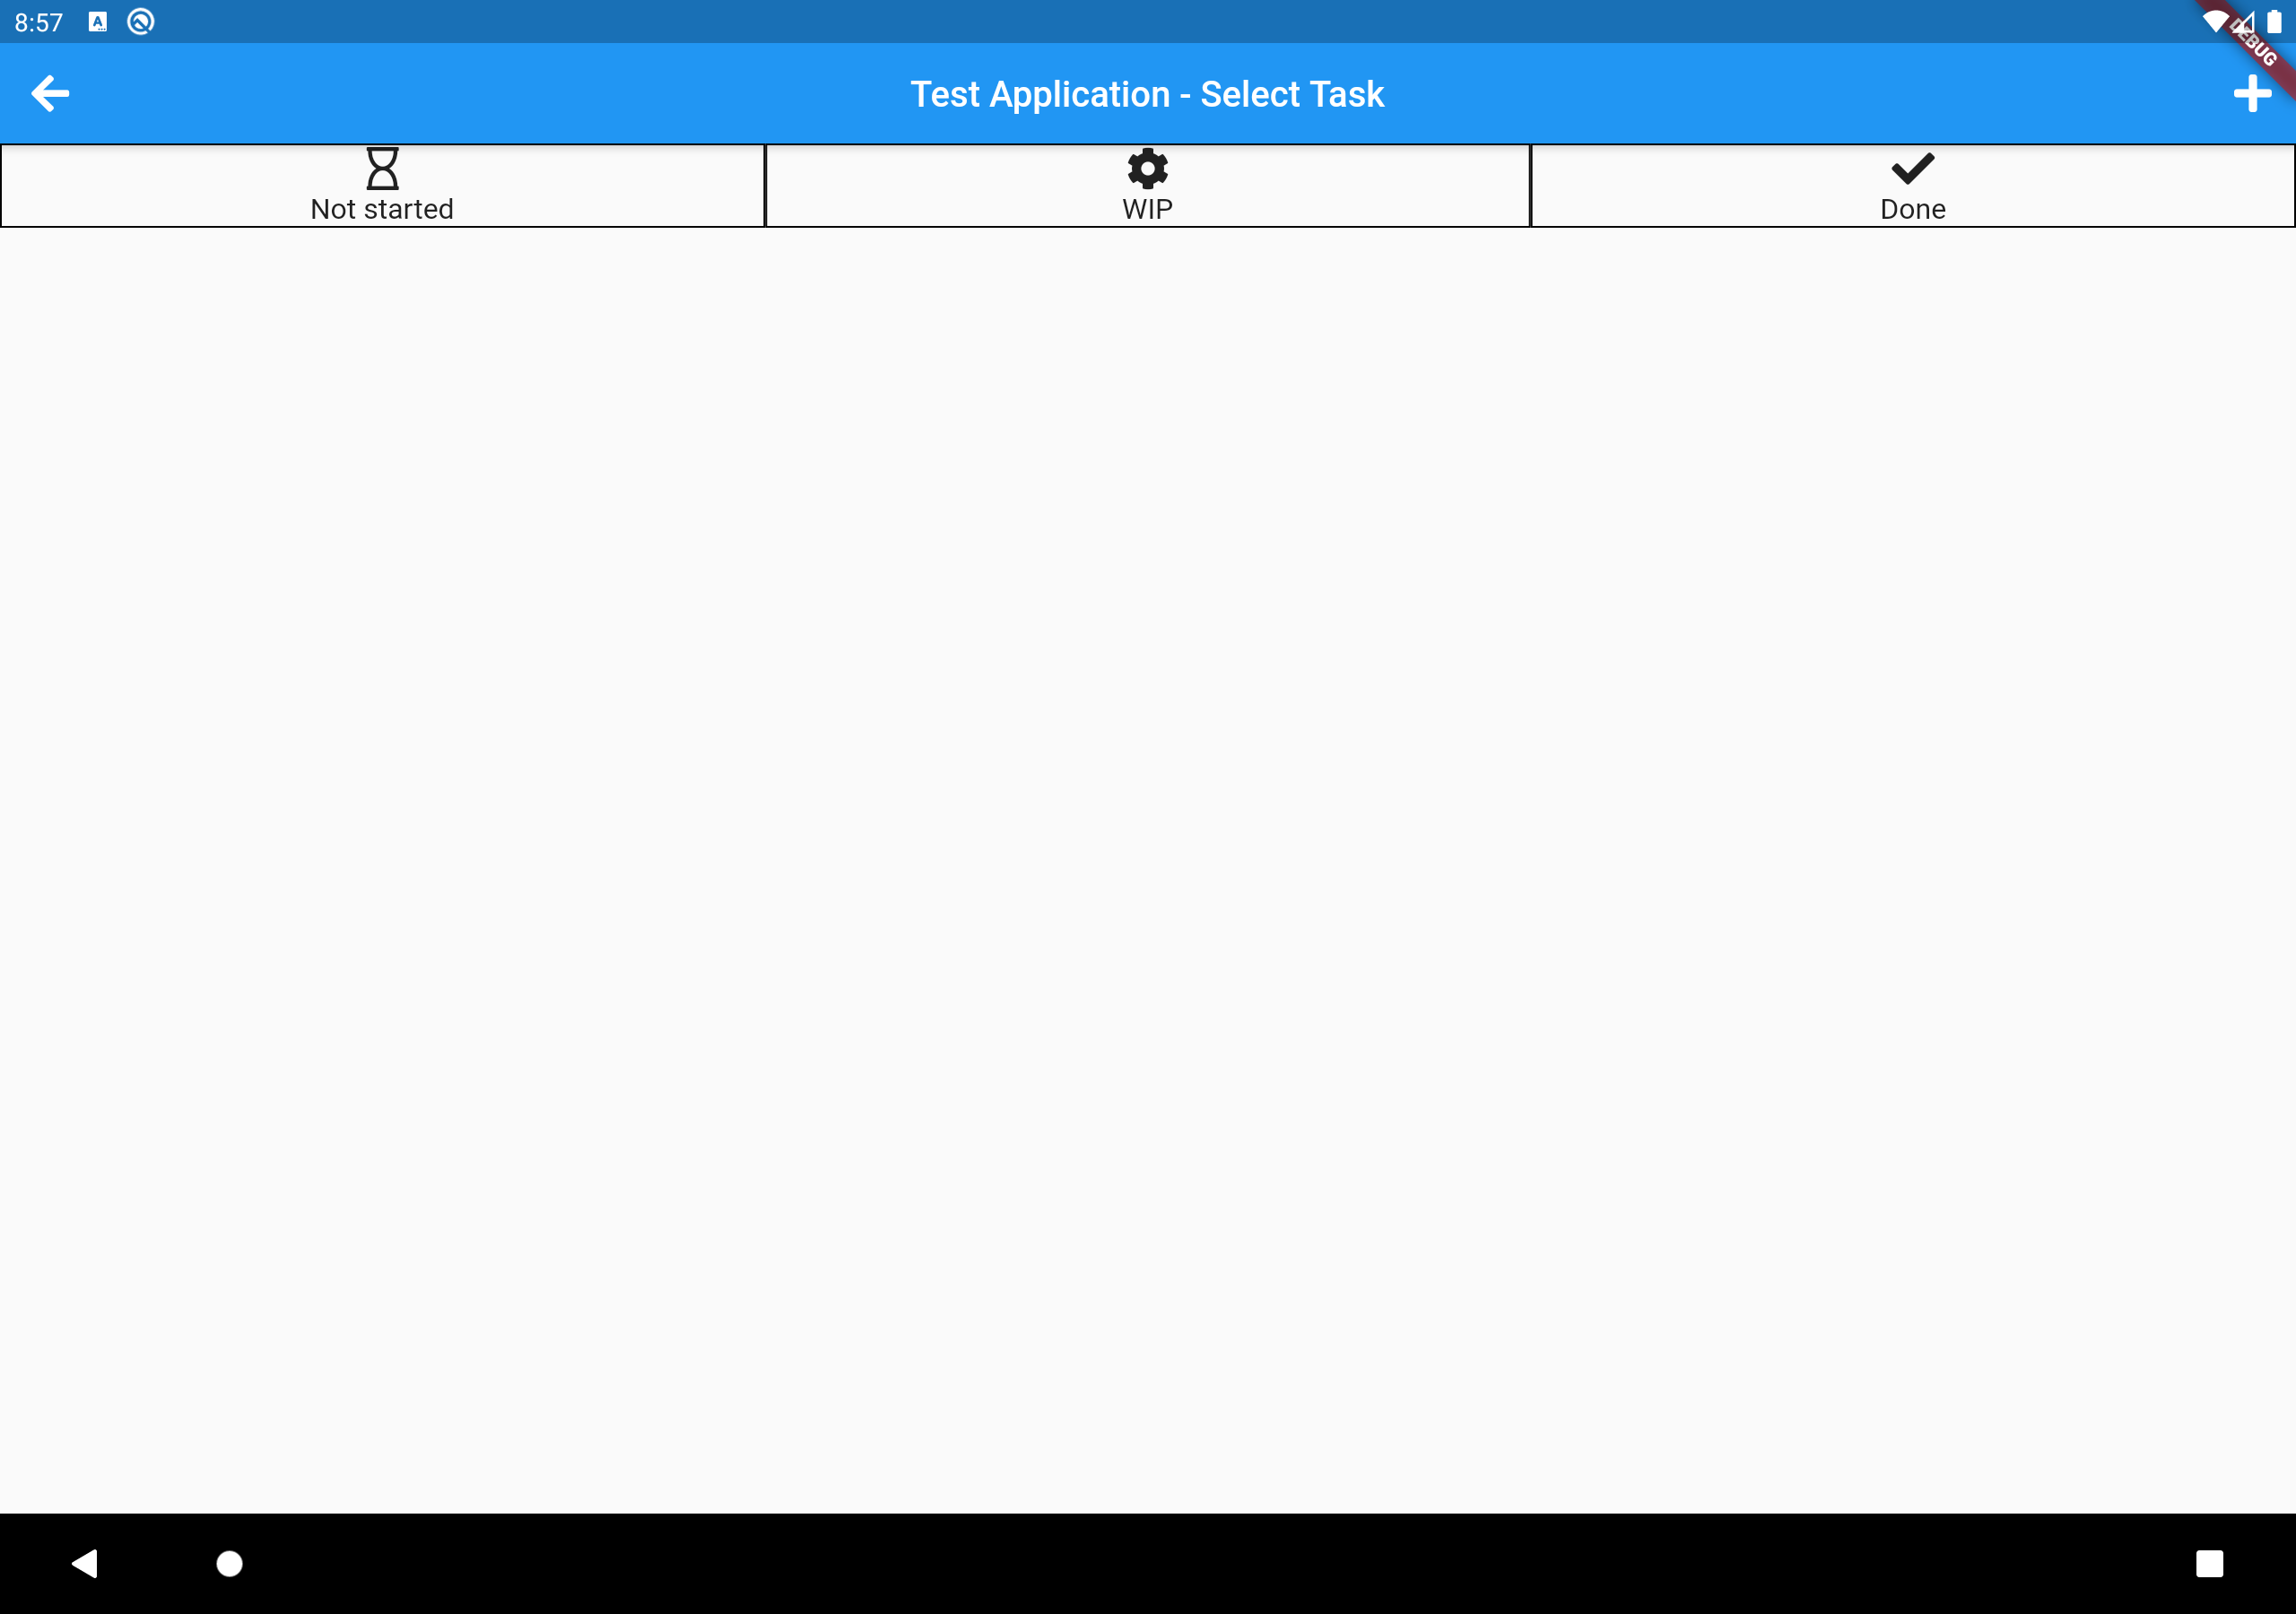
\includegraphics[width=\textwidth]{Sprint_1/images/task_dashboard_screen_app.png}
    \caption{Task dashboard screen implementation.}
    \label{task_dashboard_screen_app}
\end{figure}
